
Event-based systems are those whose architecture revolves around processing events. There are components that generate events, the channels through which the events propagate, and the listeners who react to them, potentially triggering new events too. It's a style that promotes asynchrony and loose coupling, which makes it a good way to increase performance and scalability, as well as an easy solution to deploy.

With those advantages, there are also some challenges to solve. One of them is the complexity to create a system of this type. All the queues must be made fault-tolerant so that no events are lost in the middle of being processed. Processing transactions in a distributed way is also a challenge on its own. Using the Correlation ID pattern to track events between processes, along with monitoring techniques, can save you hours of debugging and scratching your head.

Examples of event-based systems include stream processors and data integrations, as well as systems aiming for low latency or high scalability.

Let's now discuss common topologies used in such  systems.


\subsubsubsection{2.5.1\hspace{0.2cm}Common event-based topologies}

The two main topologies of event-driven architectures are broker-based and mediatorbased. Those topologies differ in how the events flow through the system.

The mediator topology is best used when processing an event that requires multiple tasks or steps that can be performed independently. All events produced initially land in the mediator's event queue. The mediator knows what needs to be done in order to handle the event, but instead of performing the logic itself, dispatches the event to appropriate event processors through each processor's event channel. 

If this reminds you of how business processes flow, then you've got good intuition. You can implement this topology in Business Process Management (BPM) or Business Process Execution Language (BPEL). However, you can also implement it using technologies such as Apache Camel, Mule ESB, and others:


\begin{center}
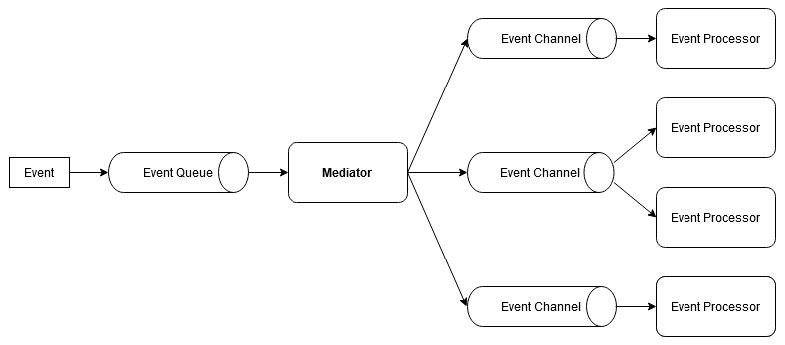
\includegraphics[width=0.9\textwidth]{content/1/chapter2/images/1.jpg}\\
Figure 2.1 – The mediator topology
\end{center}

A broker, on the other hand, is a lightweight component that contains all the queues and doesn't orchestrate the processing of an event. It can require that the recipients subscribe to specific kinds of events and then simply forwards all the ones that are interesting for them. Many message queues rely on brokers, for example, ZeroMQ, which is written in C++ and aims for zero waste and low latency:


\begin{center}
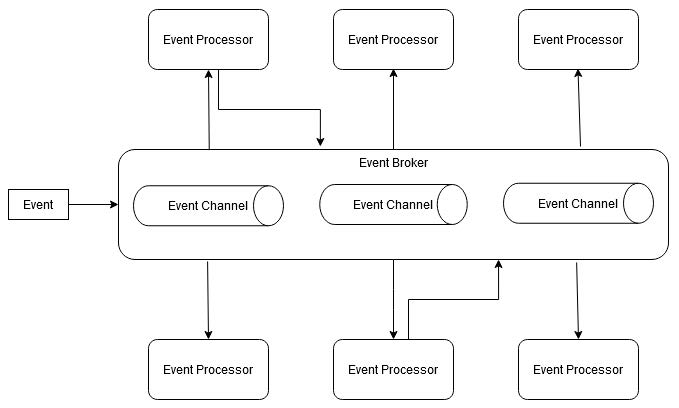
\includegraphics[width=0.9\textwidth]{content/1/chapter2/images/2.jpg}\\
Figure 2.2 – The broker topology
\end{center}

Now that you know the two common topologies used in event-based systems, let's learn about a powerful architectural pattern using events at its core.



\subsubsubsection{2.5.2\hspace{0.2cm}Event sourcing}

You can think of events as notifications that contain additional data for the notified services to process. There is, however, another way to think of them: a change of state. Think how easy it would be to debug issues with your application logic if you'd be able to know the state in which it was when the bug occurred and what change was requested of it. That's one benefit of event sourcing. In essence, it captures all the changes that happen to the system by simply recording all the events in the sequence they happened.

Often, you'll find that the service no longer needs to persist its state in a database, as storing the events somewhere else in the system is enough. Even if it does, it can be done asynchronously. Another benefit that you derive from event sourcing is a complete audit log for free:


\begin{center}
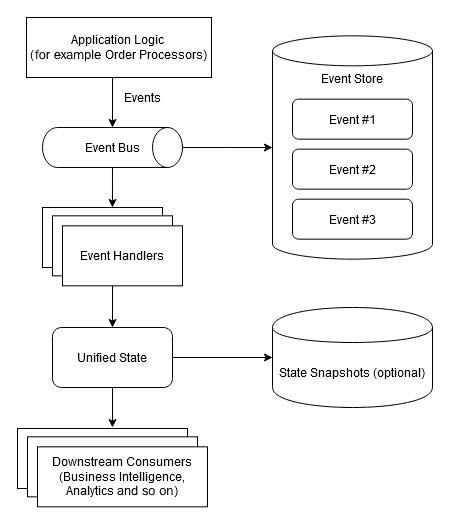
\includegraphics[width=0.9\textwidth]{content/1/chapter2/images/3.jpg}\\
Figure 2.3 – Event sourcing architecture. Providing a unified view of the application state can allow for consuming it and creating periodic snapshots for faster recovery
\end{center}

Thanks to the reduced need for data synchronization, event-sourced systems often offer low latency, which makes them a good fit for trading systems and activity trackers, among others.

Let's now learn about another popular architectural style.






















